\documentclass{article}
\usepackage{graphicx} % Required for inserting images
\usepackage[top=0.9in, bottom=1in, left=1.5in, right=1.5in]{geometry}
\usepackage[utf8]{inputenc}
\usepackage[icelandic]{babel}
\usepackage[T1]{fontenc}
\usepackage[sc]{mathpazo}
\usepackage[parfill]{parskip}
\renewcommand{\baselinestretch}{1.2}
% Tables and lists
\usepackage{booktabs,tabularx}
\usepackage{multirow}
\usepackage{enumerate}
\usepackage{adjustbox}
\usepackage{multicol}
\usepackage{xcolor}
\usepackage{algpseudocode}
\usepackage{tikz}
\usepackage{nicefrac}
\usepackage{changepage}
\usepackage{fancyvrb}
\usetikzlibrary{arrows, positioning, calc, graphs}

% Math
\usepackage{amsmath, amsfonts, amssymb, amsthm}
% Graphics

\usepackage{graphicx}
\usepackage{tikz}
% Code environment
\usepackage{minted}
%\usepackage{bm}
%\usepackage{siunitx}
%\usepackage{animate}
%\usepackage{hyperref}
%\usepackage{movie15}
%\usepackage{multicol}
%\usepackage{changepage}
\title{Gagnasafnsfræði Verkefni 3}
\author{Ragnar Björn Ingvarsson, rbi3}
\tikzset{->, >=stealth', shorten >=1pt, node distance=2cm,thick, main node/.style={circle,draw,minimum size=3em}}


\begin{document}
\renewcommand\thepage{}
	
	\maketitle

	\newpage
	\setcounter{page}{1}
	\renewcommand\thepage{\arabic{page}}

	\section{}

	\begin{itemize}
		\item[a)] 
			\begin{verbatim}
SELECT class, country
FROM Classes
WHERE numGuns > 3;
			\end{verbatim}
			\begin{center}
				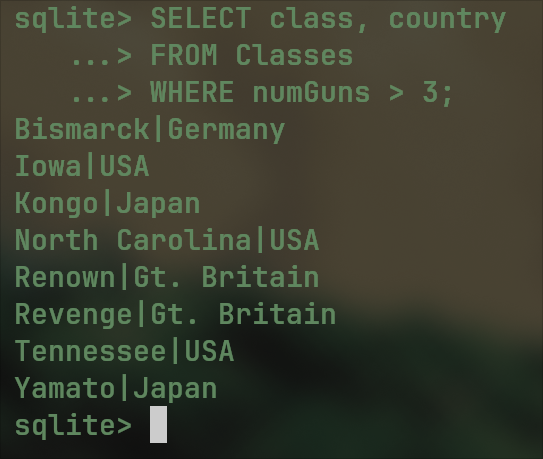
\includegraphics[scale=0.375]{numguns.png}
			\end{center}
		\item[b)] 
			\begin{verbatim}
.headers on
SELECT name AS nafn
FROM Ships
WHERE launched < 1930;
			\end{verbatim}
			\begin{center}
				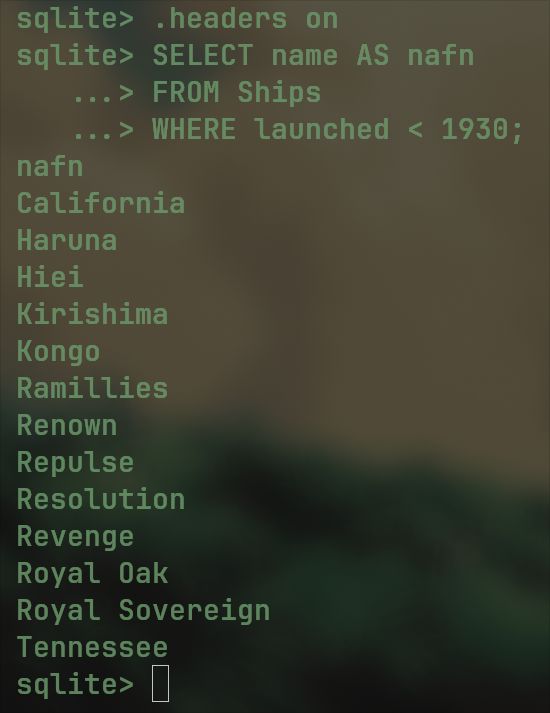
\includegraphics[scale=0.375]{launched.png}
			\end{center}
			\newpage
		\item[c)] 
			\begin{verbatim}
SELECT name
FROM Ships
WHERE name LIKE class;
			\end{verbatim}
			\begin{center}
				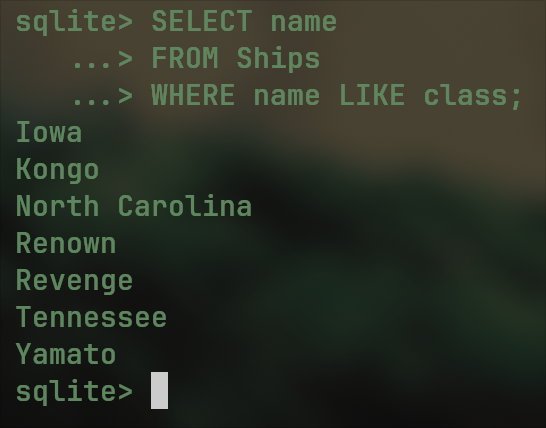
\includegraphics[scale=0.375]{likeclass.png}
			\end{center}
		\item[d)] 
			\begin{verbatim}
SELECT name
FROM Ships
WHERE name LIKE 'E%';
			\end{verbatim}
			\begin{center}
				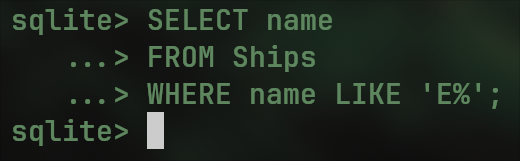
\includegraphics[scale=0.375]{estart.png}
			\end{center}
	\end{itemize}

	\newpage
	\section{}
	Hér sjáum við í fyrsta lagi að þar sem model er einstakt fyrir hverja 
	vöru, þá er model PRIMARY KEY. Við viljum svo tengja alla model dálka 
	í PC, Laptop og Printer við model dálkinn í Product með FOREIGN KEY.

	Síðan segjum við að model sé \texttt{VARCHAR(50)} og maker sé líka 
	\texttt{VARCHAR(50)}, Product.type er \texttt{VARCHAR(25)} en 
	Printer.type segjum við bara að sé \texttt{VARCHAR(30)}.

	speed er \texttt{FLOAT} þar sem það er geymt í GHz sem myndi vera 
	til dæmis 3.54GHz, ram er \texttt{INT} þar sem það er geymt í GB og 
	ekki eru seldar tölvur með 1.5GB ram eða eitthvað lengur, 
	hd er \texttt{INT} þar sem óþarfi er að mæla með nákvæmni upp á 
	kommutöluna og price er \texttt{INT} þar sem við notum íslenskar 
	krónur, og verðinu er ekki skipt í minna en eina krónu.

	Síðan viljum við að screen sé \texttt{FLOAT} þar sem við notum tommur 
	og skjástærðir eru oft t.d. $23.5"$ og color er bara \texttt{VARCHAR(30)} 
	til að gera ráð fyrir flestum litategundum.

	\begin{verbatim}
sqlite> CREATE TABLE Product (
(x1...> maker VARCHAR(50),
(x1...> model VARCHAR(50) PRIMARY KEY,
(x1...> type VARCHAR(25));
sqlite> CREATE TABLE PC (
(x1...> model VARCHAR(50) PRIMARY KEY,
(x1...> speed FLOAT,
(x1...> ram INT,
(x1...> hd INT,
(x1...> price INT,
(x1...> FOREIGN KEY (model) REFERENCES Product(model));
sqlite> CREATE TABLE Laptop (
(x1...> model VARCHAR(50) PRIMARY KEY,
(x1...> speed FLOAT,
(x1...> ram INT,
(x1...> hd INT,
(x1...> screen FLOAT,
(x1...> price INT,
(x1...> FOREIGN KEY (model) REFERENCES Product(model));
sqlite> CREATE TABLE Printer (
(x1...> model VARCHAR(50) PRIMARY KEY,
(x1...> color VARCHAR(30),
(x1...> type VARCHAR(30),
(x1...> price INT,
(x1...> FOREIGN KEY (model) REFERENCES Product(model));
\end{verbatim}

\begin{center}
	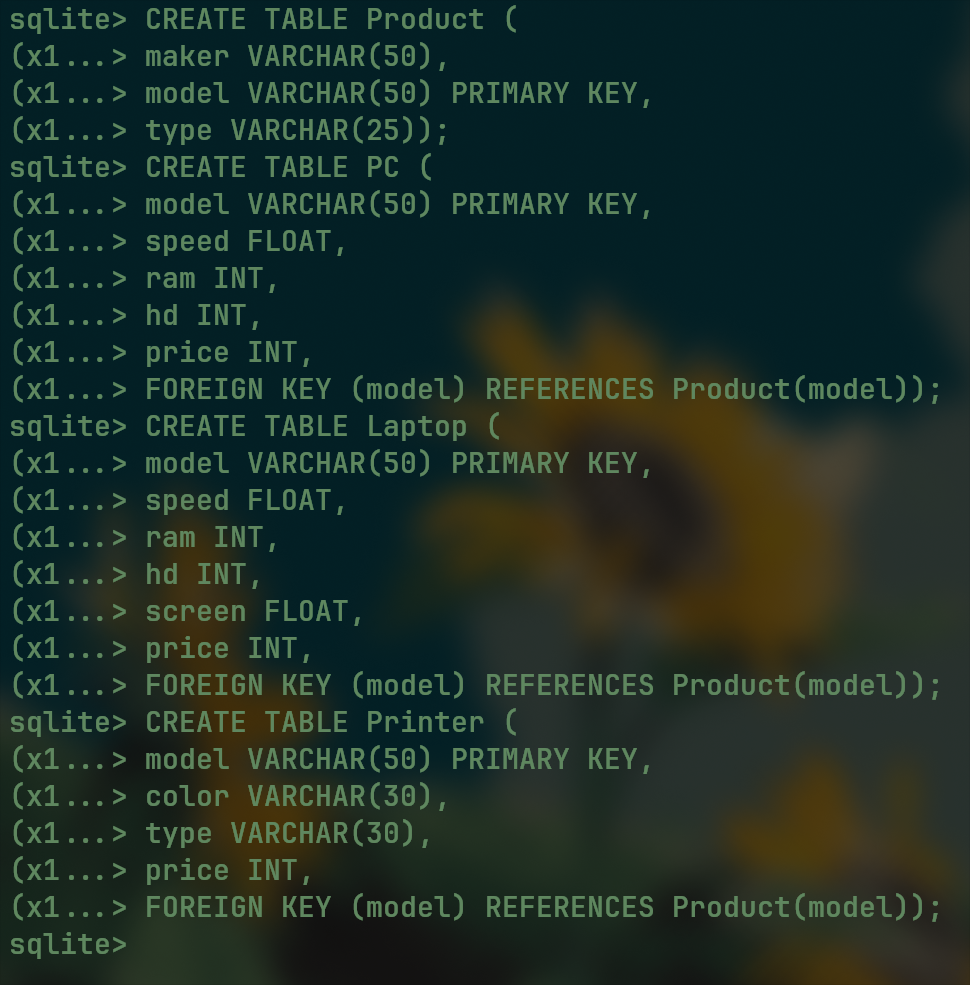
\includegraphics[scale=0.3]{db.png}
\end{center}

Og svo lítur þetta svona út í \textit{sqlitebrowser}:

\begin{center}
	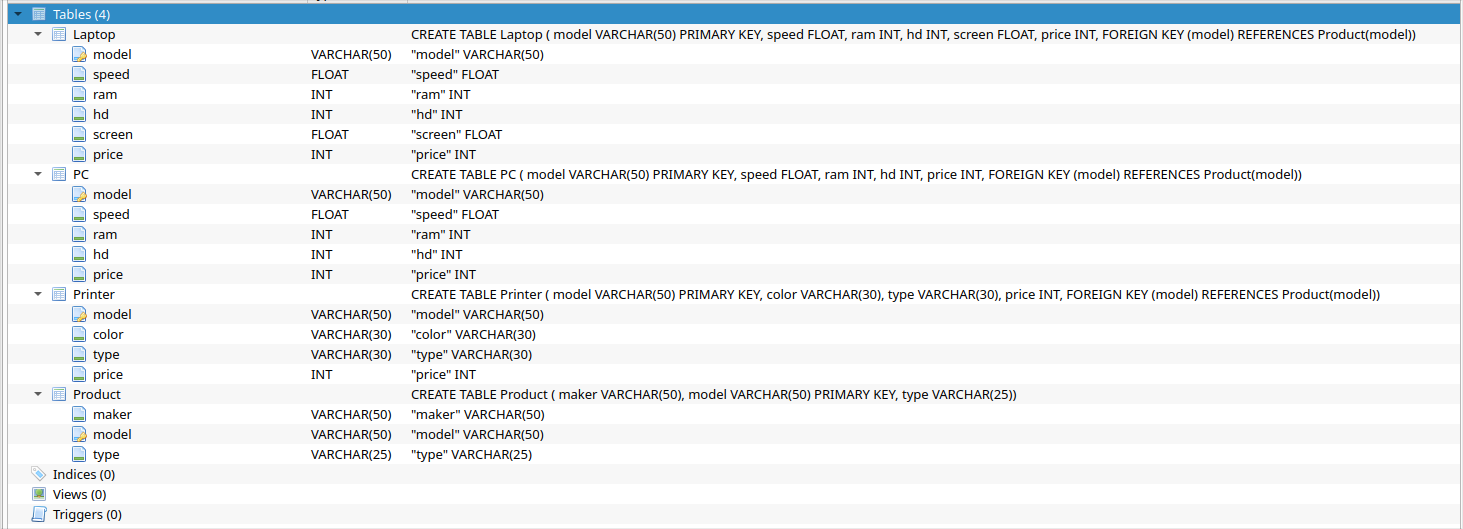
\includegraphics[scale=0.275]{dbbrowser.png}
\end{center}
	\section{}
	\begin{itemize}
		\item[a)] 
			\begin{verbatim}
SELECT name
FROM MovieStar
JOIN StarsIn ON starName = name
WHERE gender LIKE 'F' AND movieTitle LIKE 'Titanic';
			\end{verbatim}
			\begin{center}
				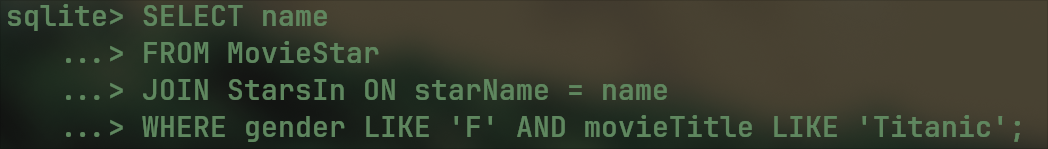
\includegraphics[scale=0.300]{titanic.png}
			\end{center}
		\item[b)] 
			\begin{verbatim}
SELECT starName
FROM StarsIn
JOIN Movie ON title = movieTitle
WHERE studioName LIKE 'Paramount' AND year = 1980;
			\end{verbatim}
			\begin{center}
				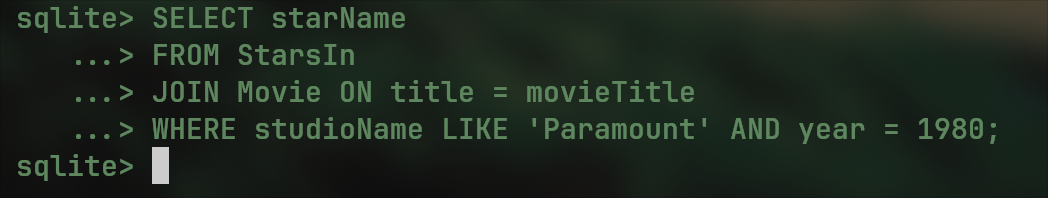
\includegraphics[scale=0.325]{1980.png}
			\end{center}
		\item[c)] 
			\begin{verbatim}
SELECT name
FROM MovieExec
JOIN Movie ON producerC = cert
WHERE studioName LIKE 'Paramount';
			\end{verbatim}
			\begin{center}
				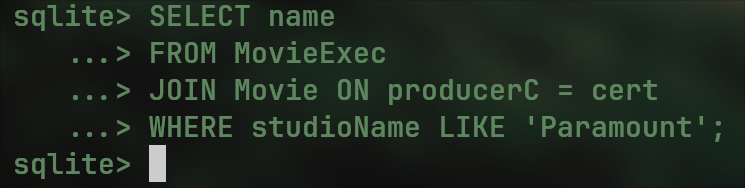
\includegraphics[scale=0.375]{parapro.png}
			\end{center}
		\item[d)] 
			\begin{verbatim}
SELECT title
FROM Movie
WHERE length >
(SELECT length FROM Movie WHERE title LIKE 'Star Wars');
			\end{verbatim}
			\begin{center}
				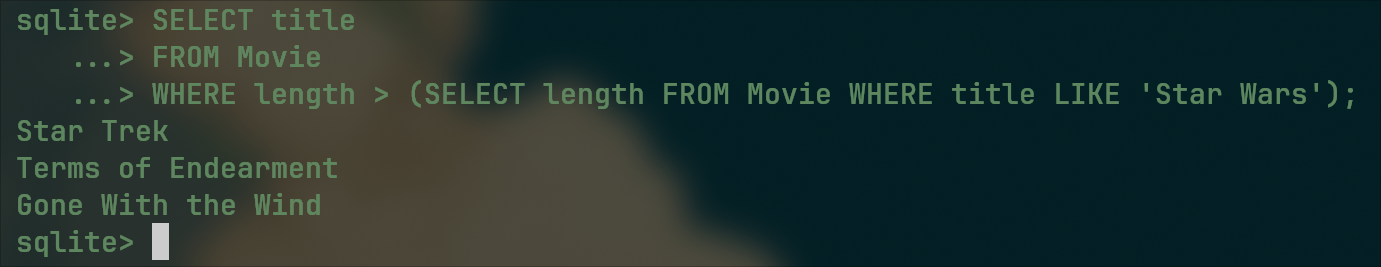
\includegraphics[scale=0.250]{starwars.png}
			\end{center}
	\end{itemize}

\end{document}
